

\lussec 9. Sample calculation in 2+1 flavour QCD

The aim in the following paragraphs is to demonstrate
the feasibility of the proposed strategies for the 
computation of the renormalization constant $\ZA$, 
the improvement coefficient $\cfl$ and the low-energy constants
$\Sigma$ and $F$. A single simulation run suffices for this
test and no attempt is made to actually compute the 
low-energy constants,
as this would require the data to be extrapolated 
to the infinite-volume, chiral and continuum limit.


\lussubsec 9.1 Simulation details

The calculations reported below are based on a
recent simulation of QCD with 2+1 flavours of quarks [\cite{TMopenQCD}].
In this run (labeled $I_1$ in ref.~[\cite{TMopenQCD}]), 
a $64\times32^3$ lattice with open boundary conditions
in time [\cite{openQCD}]
was simulated at a point in parameter space, where
the lattice spacing is estimated to be $0.090$ fm
[\cite{AokiEtAlI},\cite{AokiEtAlII}] and where 
the pion and kaon masses are about 203 and 520 MeV,
respectively [\cite{TMopenQCD}].
The physical size of the lattice is thus 
such that the finite-volume effects on the calculated 
meson masses and matrix elements are expected to be small.

For the Iwasaki gauge action [\cite{Iwasaki}]
and the standard O($a$)-improved
Wilson--Dirac operator [\cite{SW},\cite{SFimp}] used
in the simulation, the coefficients 
$\csw$ and $\ca$ are known
non-perturbatively [\cite{AokiEtAlIII},\cite{KanekoEtAl}].
A representative ensemble of 150 gauge-field configurations,
separated by $9.6$ units of molecular-dynamics time,
was produced in the run.
In order to suppress
any residual autocorrelation effects,
the statistical errors quoted in this section
were estimated by 
dividing the measurement data series for the primary observables
into bins of 5 consecutive measurements
and by applying the jackknife method to the binned data.

% Fig. 1 (converted from epsf/figure1; graphic from plots/wi.eps -> images/wi.pdf)
\topinsert
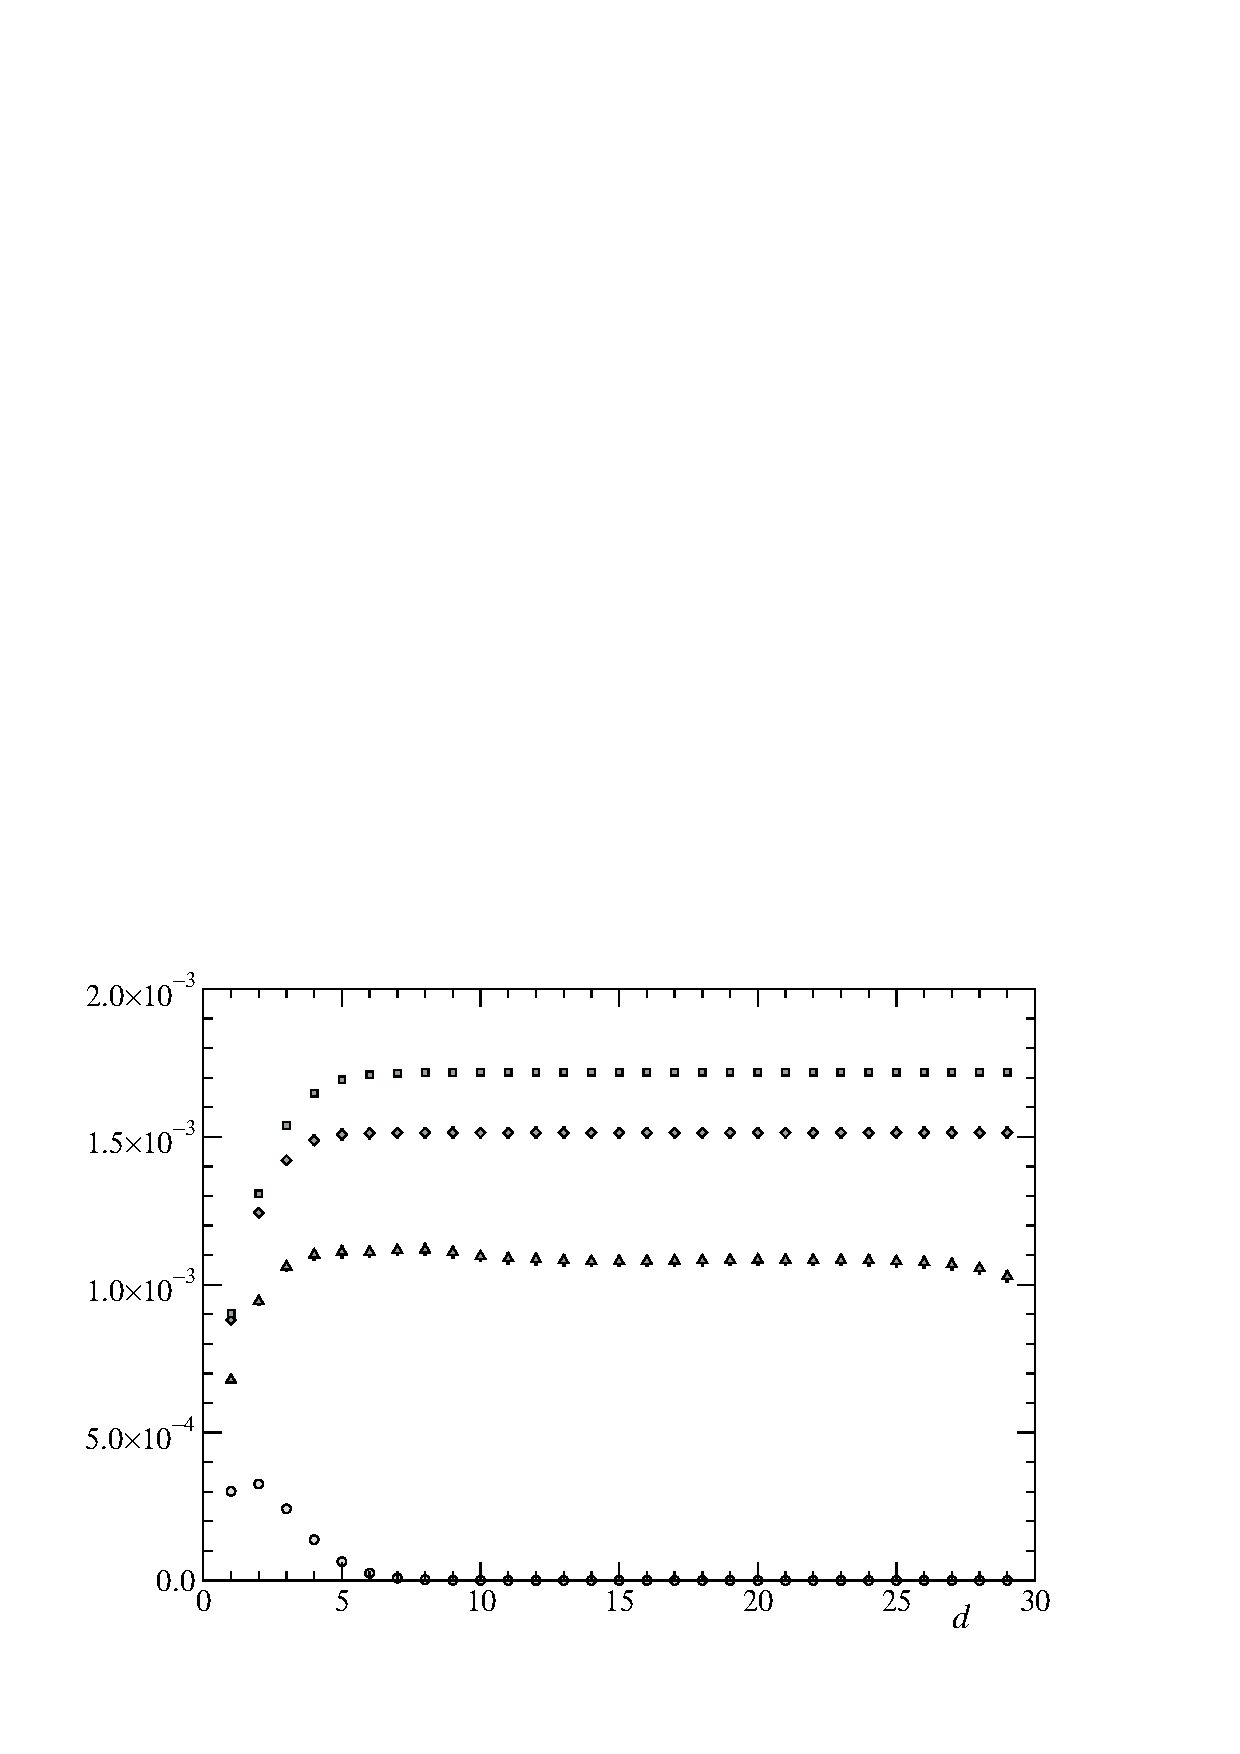
\includegraphics[width=10.5cm]{images/wi}
\vspace{0.3cm}
\figurecaption{%
Combinations of correlation functions appearing
in the PCAC relation (8.8),
plotted as a function of the summation range $d$.
The linear combinations of correlation functions shown
are the ones multiplying the renormalization constant $\ZAh{ud}$ (triangles),
the improvement coefficient $\cfl$ (diamonds)
and the factor $1-\ZAh{ud}\ctp m_{ud}$ (squares)
at flow time $t=3.86$.
For $d\geq9$, the function
$\CAtP{ud}$ (circles) is many orders of magnitude smaller than the other
functions and can be safely neglected (cf.~subsect.~8.1).
All quantities are given in lattice units.
}
\endinsert


\lussubsec 9.2 Computation of $\ZAh{rs}$ and $\cfl$

The values $2.47,\,3.86,\,5.56$ and $7.56$
of the flow time $t$ in lattice units, where
the correlation functions entering the PCAC relation (8.7)
were computed, correspond to smoothing ranges of the gradient
flow equal to $0.4,\,0.5,\,0.6$ and $0.7$ fm, respectively.
In order to keep away from the boundaries of the lattice
in the time direction, the
time-dependent field $P_t^{rs}(y)$ was inserted
in the middle of the lattice. The 
correlation functions were then averaged over space translations
using 12 random source fields at time $y_0$.

All correlation functions in the PCAC relation
can easily be obtained with small statistical errors over
the whole range of the summation window $d$.
As expected, the sum of correlation functions multiplying
the axial-current renormalization constant and the other
correlation functions reach a plateau
at values of $d$ larger than 2 or 3 times the smoothing range 
of the gradient flow (see fig.~1 for a representative case;
the slight bending down of the 
function multiplying $\ZAh{ud}$ close to the 
boundary of the lattice is a lattice-spacing effect).

Following the strategy outlined in sect.~8, the ratios (8.9)
are now determined by requiring the PCAC relation (8.8) to hold exactly 
at two values $t_1,t_2$ of $t$.
The choice of the summation window $d$ has very little influence 
on the calculated ratios as long as one stays within
the plateau range of the correlation functions.
Setting $d=18$ then leads to the results
quoted in the second and third column of table~1,
where the factor $1-\ZAh{ud}\ctp m_{ud}$ was estimated
using the tree-level value (6.22) of the coefficient $\ctp$.
As anticipated, this correction is very small (about $0.2\%$).

In the up-strange flavour channel, there are two sources of 
O($a$) mass corrections. Proceeding as above, the correction
coming from the factor $1-\ZAh{us}\ctp m_{us}$
is estimated to be approximately $1.3\%$, 
while the one deriving from the 
term in eq.~(8.10) proportional to $b_{\chi}$
changes the results by about $0.2\%$.
As can be seen from table~1,
there is a remarkable consistency among the
values of $\cfl$ obtained in the two flavour channels.
There is also little dependence on the flow
times and the difference of the renormalization constants
$\ZAh{ud}$ and $\ZAh{us}$ might very well be explained by
the mass-dependent factor in eq.~(8.4). The O($a$) improvement
thus works out very well, with residual 
lattice-spacing effects at the level of a fraction of a percent 
in the case of the renormalization constant.

\input{chapters/table1}

The results for the renormalization constant 
$\ZAh{ud}$ quoted in table~1 are in agreement
with the value $\ZA=0.781(20)$ previously
obtained in ref.~[\cite{AokiEtAlIV}]
using a method based on the Schr\"odinger functional
[\cite{ZASFI},\cite{ZASFII}]. Note that the improvement coefficient 
$\cfl$ turns out to be close to its tree-level value (6.22),
although there is no very good reason for this to be so
at the gauge coupling considered.

 
\lussubsec 9.3 Computation of the chiral condensate

Having determined the improvement coefficient $\cfl$, the unrenormalized
time-de\-pen\-dent 
condensate $\Sigma^{uu}_t$ can be computed straightforwardly
as described in subsect.~7.2.
The source time $x_0$ is taken to 
be in the middle of the lattice in order to minimize 
the excited-states contributions to the expectation value of
the scalar density. 
Using 12 random source fields, and evaluating
$\cfl$ at $t_1,t_2=3.86,5.56$, the calculation yields the results
quoted in the second column of table~2. 
In the range of flow time considered,
the time-dependent 
condensate is thus seen to decrease, roughly like $1/t$, 
when $t$ increases. The statistical error follows this
evolution and is, in any case, encouragingly small. 

\input{chapters/table2}

To be able to relate the time-dependent condensate to the 
quark condensate $\Sigma$ in the chiral limit,
the vacuum-to-pion matrix elements 
\equation{
  \Gpi=\ZP(1+b_P\mq{ud}+\bar{b}_P\tr\Mq)\kern1pt G^{ud},
  \enum
  \nexteq{3.0ex}
  \Gpit=Z_{\chi}(1+b_{\chi}\mq{ud}+\bar{b}_{\chi}\tr\Mq)\kern1pt G^{ud}_t,
  \enum
}
need to be computed as well. Actually, since only the ratio
\equation{
 {\rens{\Sigma}{t}\over\Gpit}=
 {\Sigma^{uu}_t\over G^{ud}_t}
 \enum
}
appears in eqs.~(4.24),(4.25), it suffices to calculate $\Gpi$ 
and the unrenormalized matrix element $G^{ud}_t$. The 
latter can be determined from
the pseudo-scalar correlation function (7.1) at 
large time separations $|x_0-y_0|$ in the same way as
the bare matrix element $G^{ud}$ at vanishing flow time 
is usually extracted from the ordinary pseudo-scalar two-point function.
Setting $x_0$ to a value next to the boundaries of the lattice, 
there is in all cases a wide range in time $y_0$, 
where the one-pion intermediate states dominate
and the desired matrix elements can be easily determined.

Similarly to the time-dependent condensate, the matrix element
$G^{ud}_t$ is a monotonically decreasing function of $t$.
The ratios listed in the last two columns of table~2 however
vary much less with $t$, consistently with
the fact that the flow-time dependence of the ratios must disappear
in the chiral limit.


\lussubsec 9.4 Remarks

{\it Conversion to physical units.}
The spacing 
of the simulated lattice,
$a=0.08995(40)$ fm, was determined by PACS-CS 
through a computation of the mass of the $\Omega$ baryon
[\cite{AokiEtAlII}]. Using step scaling and the Schr\"odinger functional,
PACS-CS also calculated the renormalization constant
$\ZP=0.580(21)$ [\cite{AokiEtAlIV}] 
that relates the bare matrix element $G^{ud}$ to
$\Gpi$ in the $\MSbar$ 
scheme at 2 GeV\kern1pt\sfn{$\dagger$}{%
A combination of table entries quoted in ref.~[\cite{AokiEtAlIV}],
with errors added in quadrature,
was required to obtain the value of $\ZP$ given here.}. 
At $t=3.86$, for example, the results
\equation{
  {\rens{\Sigma}{t}\Gpi\over\Gpit}=[287(4)\,\MeV]^3,
  \enum
  \nexteq{2.5ex}
  {\rens{\Sigma}{t}\over\Gpit}=91(2)\,\MeV,
  \enum
}
are then obtained, where the O($a$) mass correction in eq.~(9.1) was
neglected (the error in eq.~(9.4) is anyway dominated by 
the error of $\ZP$). Clearly, while these ratios may be close
to the condensate $\Sigma$ and decay constant $F$ in the chiral limit,
simulations of a range of lattices will be required
to be able to determine $\Sigma$ and $F$ with controlled 
systematic errors.

\vskip0.5ex
\noindent
{\it Pseudo-scalar decay constants.}
Since the calculation of the axial-current renormalization 
constant does not require separate simulations,
the renormalized pseudo-scalar meson decay constants
become directly accessible on each simulated lattice.
Depending on the flavour channel and
the precision that is to be attained,
the mass-dependent O($a$) corrections in the PCAC
relation used to determine the renormalization constant
$\ZAh{rs}$ may however need to be estimated non-perturbatively.

\vskip0.5ex
\noindent
{\it Scaling to the continuum limit.}
The results of the computations reported in this section
depend on a choice of flow times.
When lattices with different spacings are simulated,
these parameters should be held fixed
in units of a suitable reference scale such
as the reference flow time $t_0$ [\cite{WilsonFlow}].
Only then can the calculated renormalized quantities 
be expected to converge to the continuum limit
with a rate proportional to $a^2$.
